\documentclass[a4paper,14pt]{article}

\usepackage{comment} % Para comentar várias linhas ao mesmo tempo

%matemática
\usepackage{amsmath}
\usepackage{amssymb}

%diagramação
\usepackage{extsizes}
\everymath{\displaystyle}
\usepackage{geometry}
\usepackage{fancyhdr}
\usepackage{multicol}
\usepackage{graphicx}
\usepackage[brazil]{babel}
\usepackage[shortlabels]{enumitem}
\usepackage{cancel}
\usepackage{textcomp}
\usepackage{tcolorbox}

%tabelas
\usepackage{array} % Para melhor formatação de tabelas
\usepackage{longtable}
\usepackage{booktabs}  % Para linhas horizontais mais bonitas
\usepackage{float}   % Para usar o modificador [H]
\usepackage{caption} % Para usar legendas em tabelas
\usepackage{wrapfig} % Para usar tabelas e figuras flutuantes


%tikzpicture
\begin{comment}
	\usepackage{tikz}
	\usepackage{scalerel}
	\usepackage{pict2e}
	\usepackage{tkz-euclide}
	\usetikzlibrary{calc}
	\usetikzlibrary{patterns,arrows.meta}
	\usetikzlibrary{shadows}
	\usetikzlibrary{external}
\end{comment}


%pgfplots
\usepackage{pgfplots}
\pgfplotsset{compat=newest}
\usepgfplotslibrary{statistics}
\usepgfplotslibrary{fillbetween}

%colours
\usepackage{xcolor}



\columnsep=2cm
\hoffset=0cm
\textwidth=8cm
\setlength{\columnseprule}{.1pt}
\setlength{\columnsep}{2cm}
\renewcommand{\headrulewidth}{0pt}
\geometry{top=1in, bottom=1in, left=0.7in, right=0.5in}

\pagestyle{fancy}
\fancyhf{}
\fancyfoot[C]{\thepage}

\begin{document}
	
	\noindent\textbf{6FMA13 - Matemática} 
	
	\begin{center}Lendo e escrevendo (Versão estudante)
	\end{center}
	
	\noindent\textbf{Nome:} \underline{\hspace{10cm}}
	\noindent\textbf{Data:} \underline{\hspace{4cm}}
	
	%\section*{Questões de Matemática}
	
	\begin{multicols}{2}
		\noindent Para escrever qualquer número, usamos os algarismos indo-arábicos: 0, 1, 2, 3, 4, 5, 6, 7, 8 e 9. \\
		Ao expressarmos uma quantidade, podemos usar palavras da nossa língua ou esses algarismos. Para números muito grandes, é melhor a segunda opção.
		\noindent\textsubscript{-----------------------------------------------------------------------}
		\begin{enumerate} 
			\item Escreva usando numerais.
			\begin{enumerate}[a)]
				\item Dezenove. \\\\\\\\
				\item Oitenta e sete. \\\\\\\\
				\item Duzentos e noventa e seis. \\\\\\\\
				\item Dois mil, quatrocentos e cinquenta e um. \\\\\\\\
				\item Vinte mil, oitocentos e doze. \\\\\\\\
				\item Um milhão, oitocentos e quatro mil, quinhentos e trinta e dois. \\\\\\\\
			\end{enumerate}
			\item Quantos sinais diferentes usamos para representar os números? Quantos dedos você tem em suas mãos? \\\\\\\\\\\\
			\item Escreva um número com quatro algarismos iguais. \\\\\\\\
			\item Escreva um número com cinco algarismos distintos (isto é, diferentes uns dos outros). \\\\\\\\
			\item Acabe de preencher o cheque abaixo. \\
		\end{enumerate}
	\end{multicols}
	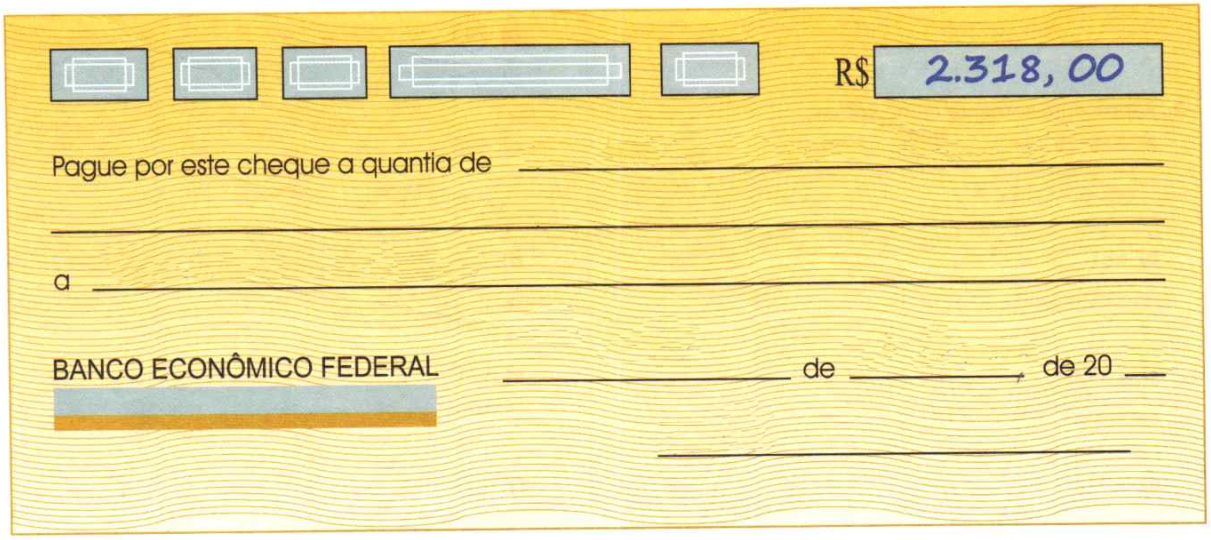
\includegraphics[width=1\linewidth]{6FMA13_imagens/imagem1}
	\begin{multicols}{2}
		\begin{enumerate}[start=6]
			%47 a 48
			\item Escreva por extenso os numerais:
			\begin{enumerate}[a)]
				\item 87 \\\\\\
				\item 365 \\\\\\\
				\item 2 438 \\\\\\
				\item 13 903 \\\\\\
				\item 2 820 071 \\\\\\\\\\
			\end{enumerate}
			\item Escreva usando numerais.
			\begin{enumerate}[a)]
				\item Noventa e três. \\\\\\
				\item Trezentos e sete. \\\\\\
				\item Quarenta e um mil e vinte e seis. \\\\\\
				\item Quatrocentos mil, duzentos e setenta e quatro. \\\\\\
				\item Três milhões e oito.
			\end{enumerate}
			$~$ \\ $~$ \\ $~$ 
		\end{enumerate}
	\end{multicols}
\end{document}